\documentclass[crop,tikz,convert=pdf2svg]{standalone}

% Tikz settings optimized for causal graphs.
\usetikzlibrary{shapes,decorations,calc,arrows.meta,fit,positioning, calligraphy}
\usepackage{pgfplots}

\begin{document}   

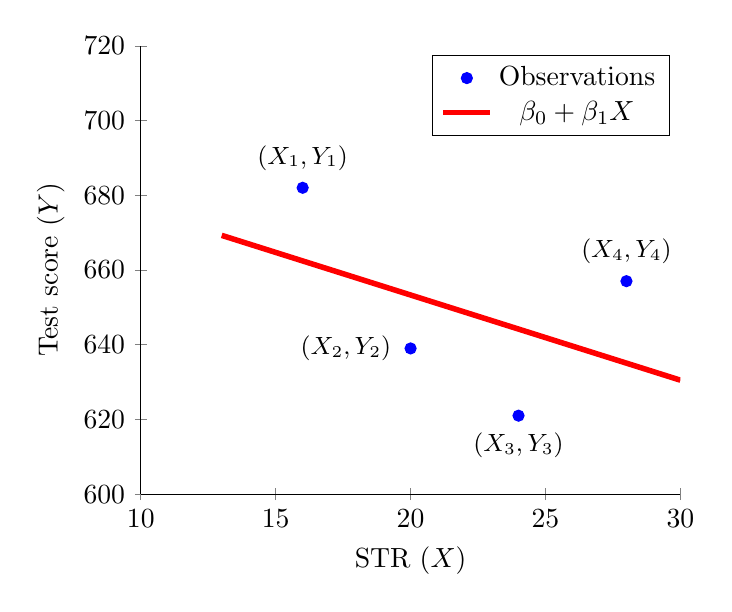
\begin{tikzpicture}

\begin{axis}[
	axis lines = left,
	axis line style = {-},
	ymin = 600,
	ymax = 720,
	xmin = 10,
	xmax = 30,
	xlabel = STR ($X$),
	ylabel = Test score ($Y$),
	]

	\addplot [
	only marks, 
	mark size = 2pt,
	color = blue, 
	] coordinates {
	(16, 682)		
	(20, 639)
	(24, 621)
	(28, 657)
	};
	\node[font=\small] at (axis cs: 16, 690) {($X_1,Y_1$)};
	\node[font=\small] at (axis cs: 17.6, 639) {($X_2,Y_2$)};
	\node[font=\small] at (axis cs: 24, 613) {($X_3,Y_3$)};
	\node[font=\small] at (axis cs: 28, 665) {($X_4,Y_4$)};
	\addlegendentry{Observations}

	% Below the red regression line is plotted
	\addplot [
	domain= 13:30,
	samples=100,
	color=red,
	line width=2pt,
	]
	{698.9 - 2.28 * x};
	\addlegendentry{$\beta_0 + \beta_1 X$}

	% \draw [decorate, decoration = {brace, mirror}] (axis cs: 16.4, 663) --  (axis cs: 16.4, 682);
	% \node[font=\small] at (axis cs: 17.2, 672) {$u_1$};
	% \draw [decorate, decoration = {brace, mirror}] (axis cs: 20.4, 639) --  (axis cs: 20.4, 651);
	% \node[font=\small] at (axis cs: 21.2, 644.5) {$u_2$};
	% \draw [decorate, decoration = {brace, mirror}] (axis cs: 24.4, 621) --  (axis cs: 24.4, 642);
	% \node[font=\small] at (axis cs: 25.2, 631.5) {$u_3$};
	% \draw [decorate, decoration = {brace}] (axis cs: 27.6, 638) --  (axis cs: 27.6, 657);
	% \node[font=\small] at (axis cs: 26.8, 647) {$u_4$};

	% \addplot [
	% domain= 13:30,
	% samples=100,
	% color=red,
	% line width=1pt,
	% dashed,
	% ]
	% {654};
	% \addlegendentry{Mean = $\bar{Y}$}

	% \draw [decorate, decoration = {brace, mirror}] (axis cs: 16.4, 654) --  (axis cs: 16.4, 682);
	% \node[font=\tiny] at (axis cs: 19.4, 668) {TS = $(Y_1 - \bar{Y})^2$};

	% \draw [decorate, decoration = {brace}] (axis cs: 15.6, 665) --  (axis cs: 15.6, 682);
	% \node[font=\tiny] at (axis cs: 12.8, 673) {RS = $(Y_1 - \hat{Y})^2$};

	% \draw [decorate, decoration = {brace}] (axis cs: 15.6, 654) --  (axis cs: 15.6, 662);
	% \node[font=\tiny] at (axis cs: 12.8, 657) {ES = $(\hat{Y} - \bar{Y})^2$};


\end{axis}
\end{tikzpicture}
\end{document}
